\documentclass[journal]{IEEEtran}

\usepackage{amsmath,amssymb}
\usepackage{graphicx}
\usepackage{cite}
\usepackage{booktabs}
\usepackage{multirow}
\usepackage{url}
\usepackage{algorithm}
\usepackage{algpseudocode}
\graphicspath{{figures/}}

\begin{document}

\title{CloudRAG: A Cloud-Native, Microservices-Based Retrieval-Augmented Generation Framework for Scalable, Secure, and Multi-Tenant Enterprise Knowledge Platforms}

\author{Aaryan~Sanjay~Paranjape, Aryan~Chandra, S.~Badri~Narayana, and Saish~Hitesh~Thakur%
\thanks{The authors are with the Manipal Institute of Technology, Manipal, India. E-mail:\newline
aaryan2.mitmpl2023@learner.manipal.edu (A.~S.~Paranjape),\newline
aryan7.mitmpl2023@learner.manipal.edu (A.~Chandra),\newline
badri.mitmpl2023@learner.manipal.edu (S.~B.~Narayana),\newline
thakur.mitmpl2023@learner.manipal.edu (S.~H.~Thakur).}%
\thanks{Student IDs: 230911168 (G022), 230911174 (G023), 230911218 (G024), 230911512 (G046).
Source code: github.com/saishthakur/cloud-native-rag.}%
}

\maketitle

\begin{abstract}
Enterprise knowledge repositories are large, heterogeneous and frequently updated, and they cannot be
accessed reliably through the parametric knowledge of a language model alone. Retrieval-augmented
generation (RAG) grounds answers in retrieved evidence, but enterprise deployment adds requirements for
independent scaling, retrieval that adapts to question complexity, tenant isolation, privacy, poisoning
resistance and observability. This paper presents the design, implementation and evaluation of CloudRAG,
a cloud-native RAG platform that decomposes the pipeline into seven independently scalable services on
Kubernetes. A query-complexity-aware router selects among naive, advanced (hybrid with reranking),
graph-augmented and agentic retrieval; a hybrid engine fuses HNSW vector search, BM25 and
relation-aware knowledge-graph traversal with reciprocal-rank fusion; and security is built into the
pipeline through tenant-sharded namespaces, chunk-level access control, ingestion-time PII redaction,
signed provenance, poisoning quarantine and a hash-chained audit log. Over five independent synthetic
multi-tenant corpora, CloudRAG reached 96.7$\pm$1.1\% answer accuracy against 92.7$\pm$1.6\% for the
strongest baseline (agentic RAG), with 2.5$\times$ lower median latency, 1.7$\times$ higher throughput
and 37\% fewer service-to-service calls. Across 120 leakage probes no cross-tenant or unauthorised
access occurred, no seeded PII reached the index, and no poisoning attack succeeded, while all
security controls together cost 12\% of ingestion time and 1.3\% of query latency.
\end{abstract}

\begin{IEEEkeywords}
Retrieval-augmented generation, cloud-native systems, microservices, knowledge graphs, multi-tenancy,
information retrieval, security, Kubernetes
\end{IEEEkeywords}

\section{Introduction}

\subsection{Background}
Organisations hold growing volumes of unstructured knowledge: documents, wikis, product sheets,
procurement records and customer interactions. Large language models (LLMs) can produce fluent answers
over such material, but they hallucinate, their parametric knowledge goes stale, and they have no access
to private data. Retrieval-augmented generation addresses these limitations by retrieving relevant
evidence first and conditioning generation on it, an approach established by Lewis \textit{et al.}
with dense retrieval over a non-parametric store~\cite{lewis2020rag}.

\subsection{Motivation}
Moving RAG from a prototype to an enterprise platform changes the problem. Corpora are large and change
continuously; many users query concurrently; questions range from single facts to multi-hop chains across
documents; different organisations (tenants) and different roles within them must never see each
other's data; personal data must be protected; and the knowledge base itself becomes an attack surface
through poisoned documents and indirect prompt injection~\cite{ammann2025securing}. Monolithic pipelines
scale as one unit, apply one retrieval strategy to every question, and treat security and monitoring as
add-ons. Cloud-native techniques---containerised services, orchestration, event-driven communication and
service-mesh governance---offer the architectural tools to address these demands together.

\subsection{Problem Statement}
Current RAG systems do not consistently combine independent scaling, adaptive retrieval, fine-grained
tenant isolation, integrated security, heterogeneous knowledge support and real-time observability.
This work asks: \emph{how can a cloud-native, microservices-based RAG framework be designed, implemented
and evaluated to achieve strong retrieval quality and answer faithfulness while supporting horizontal
scalability, multi-tenant security and cost efficiency, adapting retrieval to query complexity?}

\subsection{Research Gap}
Retrieval research has moved from single-pass pipelines to advanced, modular and agentic
designs~\cite{fan2024survey}, and graph-based methods support relational and global
questions~\cite{edge2024graphrag,barron2024domain}. However, each approach typically optimises one
dimension: agentic workflows add latency for every query, graph construction adds cost, and security and
benchmark frameworks~\cite{ammann2025securing,upadhyay2025trec} are not by themselves deployable
multi-tenant platforms. Few systems measure retrieval quality, faithfulness, latency, throughput,
communication cost and security together on one architecture.

\subsection{Objectives}
The objectives of this research are:
\begin{itemize}
    \item To design a Kubernetes-orchestrated architecture that decomposes ingestion, embedding, indexing,
          retrieval, reranking, generation and observability into independently deployable services.
    \item To develop a query-complexity-aware router that selects naive, advanced, graph-augmented or
          agentic retrieval under an optional latency budget.
    \item To implement a hybrid retrieval layer combining dense vector search, BM25 and knowledge-graph
          traversal with reciprocal-rank fusion and reranking.
    \item To engineer tenant-scoped security: namespace isolation, document- and chunk-level RBAC, PII
          redaction, provenance, poisoning detection and audit logging.
    \item To build an observability and evaluation harness, and to evaluate the platform against vanilla,
          advanced, GraphRAG and agentic RAG baselines.
\end{itemize}

\subsection{Contributions}
The contributions of this work are:
\begin{itemize}
    \item An open-source reference implementation of a seven-service RAG platform with event-driven,
          versioned ingestion, tenant-sharded indexes, and deployment artefacts for Docker Compose and
          Kubernetes (HPA, network policies, Istio mTLS and circuit breaking).
    \item A retrieval router that matches the accuracy of always-agentic retrieval while using it only for
          the questions that need it, reducing median latency by 2.5$\times$.
    \item A unified dense, sparse and relation-aware graph retrieval engine with rank fusion, reranking and
          an evidence-chaining generator for multi-hop answers.
    \item A security-first multi-tenant design whose controls are measured for effectiveness and overhead,
          including recovery from shard failure without data loss.
    \item A reproducible evaluation harness reporting quality, latency, throughput, compute, communication,
          cost and security across repeated runs.
\end{itemize}

\section{Related Work}

\subsection{Existing Approaches}
\textit{Naive and advanced RAG.} The retrieve-then-generate paradigm~\cite{lewis2020rag} retrieves the
top-$k$ passages by dense similarity. Advanced variants add query rewriting, hybrid lexical--dense
retrieval, reranking and iterative retrieval~\cite{fan2024survey}. Lexical retrieval with
BM25~\cite{robertson2009bm25} remains strong for exact identifiers, and reciprocal-rank
fusion~\cite{cormack2009rrf} is a robust way to combine heterogeneous rankers.

\textit{Graph-augmented RAG.} Hybrid systems combine vector stores with knowledge graphs to improve
multi-hop reasoning~\cite{barron2024domain}. GraphRAG builds an entity graph and community summaries to
answer local and global questions~\cite{edge2024graphrag}.

\textit{Agentic and multimodal RAG.} Agentic approaches add intent recognition, planning and tool use;
KA-RAG integrates knowledge graphs with agentic retrieval~\cite{gao2025karag}. Verification-centric and
all-in-one frameworks extend RAG to multimodal data and hallucination
mitigation~\cite{chen2025verification,guo2025raganything}.

\textit{Systems, evaluation and security.} RAG-Stack co-optimises quality and performance from the
vector-database perspective~\cite{jiang2025ragstack}; the TREC RAG track provides multifaceted
evaluation~\cite{upadhyay2025trec}; RAGAS defines reference-free metrics such as
faithfulness~\cite{es2024ragas}. PRAG addresses privacy-preserving retrieval~\cite{li2026prag}, and risk
frameworks catalogue poisoning, prompt injection and disclosure risks with
mitigations~\cite{ammann2025securing}.

\subsection{Comparative Analysis}
Table~\ref{tab:comparison} compares the capabilities of representative approaches. Each strong point
of an existing approach is a single dimension; none combines adaptive routing, graph reasoning,
multi-tenant security and operational measurement in one deployable system.

\begin{table}[!t]
\caption{Capability Comparison of Existing Approaches}
\label{tab:comparison}
\centering
\footnotesize
\setlength{\tabcolsep}{2.5pt}
\setbox0=\hbox{\begin{tabular}{lcccccc}
\toprule
Approach & Hybrid & Graph & Adaptive & Multi- & Security & Ops. \\
 & retrieval & reasoning & routing & tenant & controls & metrics \\
\midrule
Naive RAG~\cite{lewis2020rag} & -- & -- & -- & -- & -- & -- \\
Advanced RAG~\cite{fan2024survey} & \checkmark & -- & partial & -- & -- & -- \\
GraphRAG~\cite{edge2024graphrag} & -- & \checkmark & -- & -- & -- & -- \\
KA-RAG~\cite{gao2025karag} & \checkmark & \checkmark & agentic & -- & -- & -- \\
RAG-Stack~\cite{jiang2025ragstack} & \checkmark & -- & -- & -- & -- & \checkmark \\
Securing RAG~\cite{ammann2025securing} & -- & -- & -- & -- & \checkmark & -- \\
\textbf{CloudRAG} & \checkmark & \checkmark & \checkmark & \checkmark & \checkmark & \checkmark \\
\bottomrule
\end{tabular}}%
\leavevmode\ifdim\wd0>\columnwidth\relax\resizebox{\columnwidth}{!}{\box0}\else\box0\fi\par
\end{table}

\subsection{Research Gap}
Four themes emerge. Retrieval is moving towards adaptive strategies, but adaptivity is rarely tied to
cost and latency budgets. Knowledge graphs complement vectors for relational questions, at extra
construction cost. Security and privacy are usually analysed separately from the retrieval system. And
evaluation rarely measures quality, performance, cost and security jointly. CloudRAG targets these gaps
by evaluating the architecture as a whole.

\section{System Model and Problem Formulation}

\subsection{System Model}
The platform serves a set of tenants $\mathcal{T}$. Each tenant $t$ owns a document collection $D_t$ and
a set of principals (users) $u$ with roles $\rho(u)$ and clearance $\lambda(u)$. Documents are split into
chunks $c$, each carrying a list of access policies $A(c)$, a trust value $\tau_c\in[0,1]$ and a
provenance signature. Services communicate over authenticated HTTP; ingestion is decoupled from
indexing by a durable event stream. Indexes are partitioned into shards, and each tenant maps to one
shard via $\mathrm{shard}(t)=H(t)\bmod N$, where $H$ is SHA-256.

\textit{Assumptions.} Signing keys are kept in a secret store; client traffic uses TLS; the
orchestrator restarts failed pods; and documents may come from both systems of record and untrusted
uploads.

\textit{Threat model.} An adversary may be an authenticated user of another tenant, a user without a
required role, an insider who uploads poisoned documents, a client that submits injection queries, or an
attacker who modifies stored index content.

\subsection{Problem Formulation}
Let $S=\{\text{naive},\text{advanced},\text{graph},\text{agentic}\}$ be the retrieval strategies, with
expected cost $C(s)$, observed 95th-percentile latency $L_{95}(s)$ and expected answer quality
$Q(s,q)$ for query $q$. For each query the platform selects
\begin{equation}
    s^{*}(q)=\arg\min_{s\in S} C(s)\quad \text{s.t.}\quad Q(s,q)\ge \theta,\;\; L_{95}(s)\le B,
\end{equation}
where $\theta$ is a target quality and $B$ an optional latency budget, subject to the isolation constraint
that every retrieved chunk satisfies
\begin{equation}
    \mathrm{tenant}(c)=\mathrm{tenant}(u)\;\wedge\;\bigwedge_{p\in A(c)} \mathrm{allow}(u,p).
\end{equation}
Because $Q(s,q)$ is unknown at query time, the router approximates it from query features
(Section~\ref{sec:math}).

\section{Proposed Methodology}

\subsection{System Architecture}
Fig.~\ref{fig:architecture} shows the architecture. The \emph{gateway} authenticates JSON Web Tokens,
applies per-tenant token-bucket rate limits, filters adversarial queries, orchestrates calls and writes
the audit log. \emph{Ingestion} validates and transforms documents and publishes versioned events to
Redis Streams. \emph{Indexing} shards consume the stream, call the \emph{embedding} service and maintain
per-tenant HNSW, BM25 and knowledge-graph indexes. \emph{Retrieval} hosts the router and strategies,
calling \emph{embedding}, \emph{indexing} and the \emph{reranker} in parallel. \emph{Generation} produces
cited answers using Claude, with an offline extractive generator as fallback. Every service exports
Prometheus metrics and health probes. The user's token is forwarded on every hop and re-verified by each
service.

\begin{figure}[!t]
    \centering
    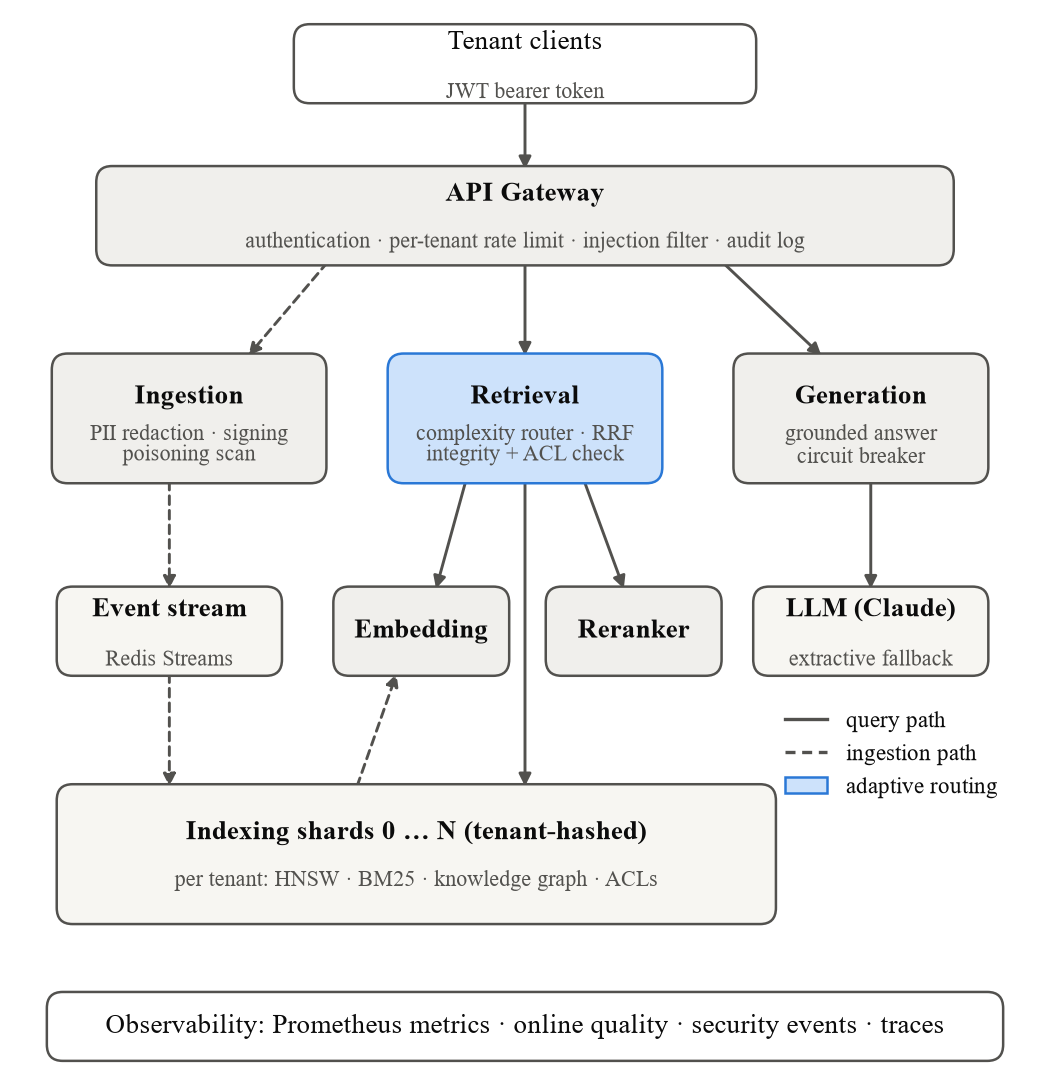
\includegraphics[width=\columnwidth]{system_architecture.png}
    \caption{Architecture of CloudRAG. Solid arrows: query path; dashed arrows: event-driven ingestion
    path. The highlighted retrieval service hosts the adaptive router.}
    \label{fig:architecture}
\end{figure}

\subsection{Proposed Framework}
\textit{Ingestion pipeline.} For each document the ingestion service (i) computes document-level poisoning
signals (hidden Unicode and near-duplicate floods via SimHash~\cite{charikar2002simhash}); (ii) removes
invisible characters and redacts PII---e-mail, phone, Luhn-validated card numbers, SSN, Aadhaar, PAN, IBAN
and IP addresses---or replaces it with keyed pseudonyms; (iii) splits text into sentence-aligned chunks of
about 120 words, never crossing inline access-controlled sections; (iv) scores each chunk for
poisoning, quarantining or down-weighting it; (v) assigns a source-based trust ceiling; (vi) signs each
chunk; and (vii) publishes a versioned upsert event. Ingestion returns immediately, so write bursts do not
affect query serving. Upserts carry a nanosecond version, making replays idempotent and stale events
harmless.

\textit{Indexing.} Each shard keeps, per tenant, an HNSW graph~\cite{malkov2020hnsw}, an incremental BM25
index, and a knowledge graph whose entities and predicate-labelled relations are extracted from chunk
text. Graph communities are found with label propagation~\cite{raghavan2007lpa}. Access policies are
evaluated as a filter \emph{during} search. Shards snapshot their namespaces together with the last
processed stream offset; after a crash they restore the snapshot and replay the stream from that offset.

\textit{Query pipeline.} After the gateway's checks, the retrieval service links entities in the
question, the router selects a strategy, retrievers run in parallel, results are fused and reranked, and
every chunk is re-verified for tenant, access policy and signature before generation. Context passages
are sanitised of instruction-like sentences and wrapped as untrusted documents. The answer cites its
sources, and the gateway computes online faithfulness and relevance estimates.

\subsection{Algorithm}
Algorithm~\ref{alg:route} summarises routing and the agentic pathway.

\begin{algorithm}[!t]
\caption{Adaptive routing and agentic retrieval}
\label{alg:route}
\footnotesize
\begin{algorithmic}[1]
\Require query $q$, principal $u$, top-$k$, budget $B$
\State $E \gets \textsc{LinkEntities}(q)$;\; $\phi \gets \textsc{Features}(q,E)$
\If{$\phi.\text{multipart}\ge 1$ \textbf{or} $\phi.\text{relational}\wedge\phi.\text{verbs}\ge 3$} $s\gets$ agentic
\ElsIf{$\phi.\text{relational}$ \textbf{or} $\phi.\text{global}$} $s\gets$ graph
\ElsIf{$\phi.\text{terms}\le 6 \wedge |E|\le 1$} $s\gets$ naive
\Else\ $s\gets$ advanced
\EndIf
\While{$B$ given \textbf{and} $L_{95}(s)>B$ \textbf{and} $s\ne$ naive} $s\gets \textsc{Cheaper}(s)$
\EndWhile
\If{$\phi.\text{global}$} $k\gets 2k$ \Comment{aggregation needs every instance}
\EndIf
\If{$s=$ agentic}
  \State $\mathcal{L}\gets\{\textsc{GraphHybrid}(q_i,k) : q_i\in \textsc{Decompose}(q)\}$
  \For{$h=1$ \textbf{to} $3$}
    \State $(\gamma, M)\gets \textsc{Coverage}(q,\mathcal{L})$
    \If{$\gamma\ge 0.85$ \textbf{and} $h>1$} \textbf{break} \EndIf
    \State $e\gets \textsc{BridgeEntity}(\text{latest hits})$ \Comment{connected, unseen}
    \State $\mathcal{L}\gets \mathcal{L}\cup \{\textsc{GraphHybrid}(e \Vert M,k)\}$
  \EndFor
  \State $R\gets \textsc{Rerank}(q,\textsc{RRF}(\mathcal{L}))$ keeping each list's top hit
\Else\ $R\gets \textsc{Run}_s(q,k)$
\EndIf
\State \Return $\{c\in R : \textsc{Verify}(c)\wedge \mathrm{tenant}(c)=\mathrm{tenant}(u)\wedge \mathrm{read}(u,c)\}$
\end{algorithmic}
\end{algorithm}

\subsection{Mathematical Model}
\label{sec:math}
\textit{Router.} From $n_t$ content terms, $n_e$ linked entities, relational cue $r$, relation verbs $v$,
aggregation cue $g$, sub-questions $m$ and comparison cue $c$, a complexity score is reported as
\begin{equation}
\begin{split}
\kappa(q)=\min\big(1,\;&0.04n_t+0.1\min(n_e,4)+0.25r+0.1\min(v,3)\\
&+0.2g+0.3\min(m,2)+0.2c\big).
\end{split}
\end{equation}

\textit{Sparse retrieval.} BM25~\cite{robertson2009bm25} with $k_1=1.2$, $b=0.75$:
\begin{equation}
\mathrm{BM25}(q,d)=\sum_{t\in q}\mathrm{idf}(t)\frac{f_{t,d}(k_1+1)}{f_{t,d}+k_1\big(1-b+b\frac{|d|}{\overline{|d|}}\big)}.
\end{equation}

\textit{Graph traversal.} Starting from linked entities with score 1, a neighbour $v'$ of $v$ over edge
$e$ receives
\begin{equation}
\sigma(v')=\sigma(v)\,\delta\,\min\!\big(1,0.6+0.2\ln(1+w_e)\big)\,\rho_e,
\end{equation}
with decay $\delta=0.5$, edge weight $w_e$, and $\rho_e=1$ if the edge predicate shares a term with the
question's relation words and $0.5$ otherwise. A chunk $c$ scores
$\sum_{v\ni c}\sigma(v)/(1+\ln(1+|C_v|))$ plus a bonus for edges whose both endpoints were reached.

\textit{Fusion and reranking.} Rankings from retrievers $r$ are combined by reciprocal-rank
fusion~\cite{cormack2009rrf}:
\begin{equation}
\mathrm{RRF}(d)=\sum_{r} \frac{w_r}{60+\mathrm{rank}_r(d)},
\end{equation}
with $w_{\text{graph}}=1.3$. The reranker scores each pair by weighted term coverage, best-sentence
coverage, bigram overlap and title match, scaled by $(0.5+0.5\tau_c)$, and the final score blends
normalised rerank and fusion scores, $s=\alpha\hat{r}+(1-\alpha)\hat{f}$, with $\alpha=0.8$ (advanced),
$0.6$ (graph) and $0.5$ (agentic).

\textit{Generation.} The default generator builds an evidence chain per sub-question: the first sentence
maximises trust-weighted, IDF-weighted support, and each further sentence must share an entity with the
chain and add uncovered question terms. This composes multi-hop answers such as ``Project~X uses
P'' $\rightarrow$ ``P is supplied by V'' $\rightarrow$ ``V is headquartered in C''.

\subsection{Security and Performance Model}
\textit{Poisoning risk.} Signals $i$ with weights $w_i$ (instruction override 0.9, exfiltration 0.85,
markup injection 0.7, hidden Unicode 0.6, keyword stuffing 0.5, near-duplicate flood 0.4, among others)
are combined by a noisy-OR,
\begin{equation}
R=1-\prod_i (1-w_i),
\end{equation}
quarantining chunks with $R\ge0.70$ and indexing chunks with $0.35\le R<0.70$ at trust
$\tau_c=\min(\tau_{\text{src}},1-R)$, where $\tau_{\text{src}}$ is the source trust ceiling (0.6 for
uploads, 1.0 for systems of record).

\textit{Integrity and auditability.} Each chunk with text $x_c$ carries the signature
\begin{equation}
\sigma_c=\mathrm{HMAC}_K\big(t\Vert d\Vert c\Vert \mathrm{SHA256}(x_c)\Vert A(c)\Vert \mathrm{src}\Vert\tau_c\big),
\end{equation}
which is verified before generation. Audit records form a hash chain
$h_i=\mathrm{SHA256}(h_{i-1}\Vert e_i)$, so any edit, deletion or reordering is detectable.

\textit{Performance model.} Per-query cost is measured as wall-clock latency, CPU time $T_{\text{cpu}}$,
internal requests and bytes, and estimated energy $E=T_{\text{cpu}}\,P_{\text{core}}$, where
$P_{\text{core}}=2.5$\,W (15\,W processor base power over six cores). LLM cost is estimated from prompt and answer
length at Claude Opus 5.5 list prices (\$4 and \$20 per million input and output tokens).

\section{Experimental Setup}

\subsection{Dataset}
Public RAG benchmarks do not provide multi-tenant corpora with role-restricted content, seeded PII and
poisoning attacks, so a deterministic synthetic enterprise corpus was generated. Each tenant has vendors,
products, projects and employees whose facts are spread across separate documents (vendor profiles,
product sheets, project charters with finance-only budget sections, HR records with contact details), plus
distractor documents. Questions have gold answers and gold evidence documents in five types:
\emph{single-hop} (one document), \emph{relational} (two documents), \emph{multi-hop} (three documents),
\emph{multi-part} (two independent facts) and \emph{aggregation} (all projects linked to a vendor).
Security probes include role-restricted questions, questions about another tenant's facts, injection
queries, benign queries, and three types of poisoned documents. Five independent corpora were generated
(seeds 7, 11, 23, 42 and 2026). Table~\ref{tab:dataset} gives the composition.

\begin{table}[!htbp]
\centering
\caption{Evaluation Corpus (per seed)}
\label{tab:dataset}
\footnotesize
\begin{tabular*}{\columnwidth}{@{\extracolsep{\fill}}lr@{}}
\toprule
Property & Value \\
\midrule
Tenants & 3 \\
Documents & 768 \\
Chunks & 816 \\
Distractor documents per tenant & 200 \\
\midrule
Single-hop questions & 24 \\
Relational questions & 12 \\
Multi-hop questions & 12 \\
Multi-part questions & 12 \\
Aggregation questions & 9 \\
Total questions & 69 \\
Seeds (independent corpora) & 5 \\
\bottomrule
\end{tabular*}
\end{table}


\subsection{Simulation/Testbed}
\begin{itemize}
    \item Hardware: 12th Gen Intel(R) Core(TM) i3-1215U (6 cores, 8 threads), 7.7 GB RAM
    \item Operating System: Windows 11
    \item Programming Language: Python 3.14.0
    \item Simulation Platform: CloudRAG in-process deployment (all seven services, in-memory event bus); distributed deployment on Docker Compose with Redis Streams and two index shards
    \item Software Tools: FastAPI, Uvicorn, NumPy, Pydantic, Redis 7.4, Docker 29, Kubernetes manifests (kustomize), Prometheus
\end{itemize}

The baselines are implemented on the same platform, sharing ingestion, indexes and generator, so that
differences reflect the retrieval pathway only: vanilla RAG (dense top-$k$), advanced RAG (dense + BM25 +
RRF + rerank), GraphRAG (graph local search + community search) and agentic RAG (always decompose and
iterate).

\subsection{Parameter Settings}
Table~\ref{tab:parameters} lists the parameters used in all experiments.

\begin{table}[!htbp]
\centering
\caption{Experimental Parameters}
\label{tab:parameters}
\footnotesize
\begin{tabular*}{\columnwidth}{@{\extracolsep{\fill}}lr@{}}
\toprule
Parameter & Value \\
\midrule
Retrieved chunks per query ($k$) & 5 \\
Chunk size & 120 words, 1-sentence overlap \\
Embedding & feature hashing, 512 dims \\
HNSW ($M$, $ef_{c}$, $ef_{s}$) & 16, 80, 64 \\
BM25 ($k_1$, $b$) & 1.2, 0.75 \\
RRF constant & 60 \\
Candidate pool & $\max(4k, 20)$ \\
Graph traversal depth & 2 hops, decay 0.5 \\
Agentic max. bridging steps & 3 \\
Quarantine / flag threshold & 0.70 / 0.35 \\
Query block threshold & 0.80 \\
Concurrent clients (throughput) & 8 \\
Repetitions & 5 independent seeds \\
Cost model & Claude Opus 5.5 list price \\
Energy model & 2.5 W per busy core \\
\bottomrule
\end{tabular*}
\end{table}


\subsection{Evaluation Metrics}
\label{sec:metrics}
The approach is evaluated using the following metrics; all are reported as mean $\pm$ sample standard
deviation over the five seeds.
\begin{itemize}
    \item \textbf{Accuracy}: share of gold answer strings contained in the generated answer (partial
          credit for multi-part and aggregation questions).
    \item \textbf{Precision, Recall, F1}: retrieval precision@$k$ (share of retrieved documents that are
          gold evidence), recall (share of gold documents retrieved) and their harmonic mean; also hit
          rate, MRR and rank-weighted context precision.
    \item \textbf{Faithfulness and relevance}: share of answer sentences supported by a context sentence,
          and question--answer embedding similarity (lexical RAGAS-style estimators~\cite{es2024ragas}).
    \item \textbf{Latency}: p50, p95 and p99 end-to-end query time.
    \item \textbf{Throughput}: queries per second with eight concurrent clients after warm-up.
    \item \textbf{Energy consumption}: estimated from CPU time as defined above.
    \item \textbf{Computational and communication overhead}: CPU time per query, index memory,
          service-to-service requests and bytes per query, and processing time of each security control.
    \item \textbf{Security}: leakage rates, PII residue, injection block and false-positive rates,
          poisoning quarantine and attack success, and audit-chain integrity.
\end{itemize}

\section{Results and Discussion}

\subsection{Performance Results}
Fig.~\ref{fig:performance}(a) shows accuracy by question type. All methods answer single-hop questions;
vanilla and advanced RAG fail relational and multi-hop questions because the second and third evidence
documents share few words with the question. GraphRAG answers relational questions (98.3\%) but not
three-hop chains (8.3\%). Agentic RAG answers every type except aggregation (31.1\%). CloudRAG matches the
best method on single-hop, relational, multi-hop and multi-part questions (100\%) and reaches 69.4\% on
aggregation, where the router doubles the context budget. Table~\ref{tab:bytype} gives the values and
Table~\ref{tab:retrieval} the retrieval metrics.

\begin{figure}[!t]
    \centering
    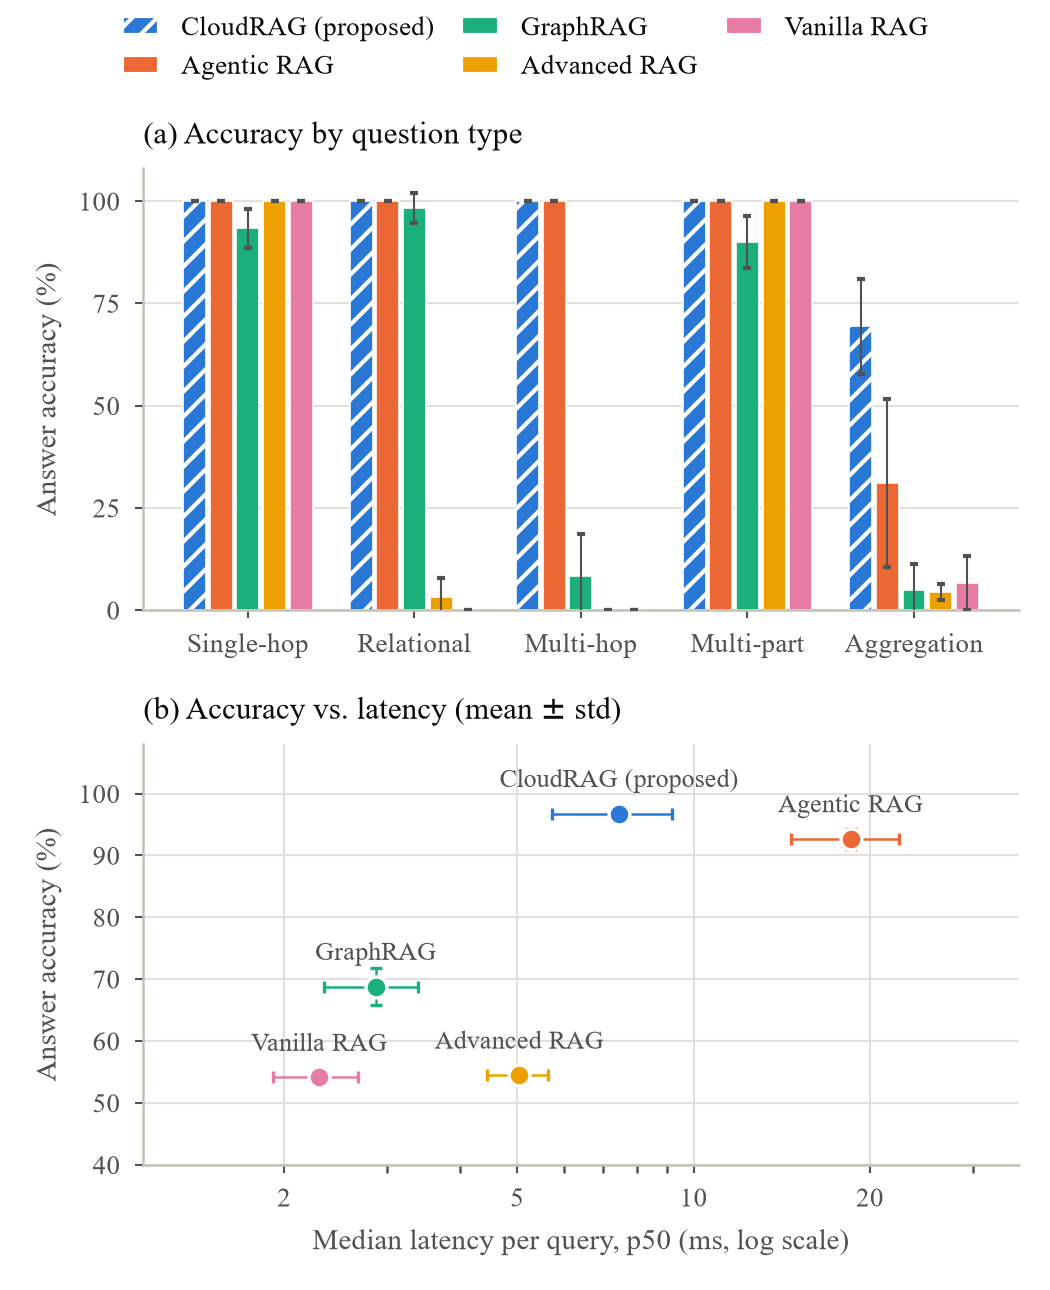
\includegraphics[width=\columnwidth]{performance_results.png}
    \caption{Performance of CloudRAG and the baselines over five seeds: (a) answer accuracy by question
    type; (b) accuracy against median latency.}
    \label{fig:performance}
\end{figure}

\begin{table}[!t]
\caption{Answer Accuracy (\%) by Question Type}
\label{tab:bytype}
\centering
\footnotesize
\setlength{\tabcolsep}{3pt}
\setbox0=\hbox{\begin{tabular}{lccccc}
\toprule
Method & Single-hop & Relational & Multi-hop & Multi-part & Aggregation \\
\midrule
Vanilla RAG & 100.0 & 0.0 & 0.0 & 100.0 & 6.6 \\
Advanced RAG & 100.0 & 3.3 & 0.0 & 100.0 & 4.4 \\
GraphRAG & 93.3 & 98.3 & 8.3 & 90.0 & 4.9 \\
Agentic RAG & 100.0 & 100.0 & 100.0 & 100.0 & 31.1 \\
CloudRAG (proposed) & 100.0 & 100.0 & 100.0 & 100.0 & 69.4 \\
\bottomrule
\end{tabular}}%
\leavevmode\ifdim\wd0>\columnwidth\relax\resizebox{\columnwidth}{!}{\box0}\else\box0\fi\par
\end{table}

\begin{table*}[!t]
\caption{Retrieval and Generation Quality (mean over seeds)}
\label{tab:retrieval}
\centering
\footnotesize
\setlength{\tabcolsep}{3pt}
\setbox0=\hbox{\begin{tabular}{lcccccc}
\toprule
Method & Hit@k & MRR & Ctx-P & Ctx-R & Faith. & Rel. \\
\midrule
Vanilla RAG & 0.950 & 0.909 & 0.885 & 0.711 & 1.000 & 0.598 \\
Advanced RAG & 0.905 & 0.894 & 0.848 & 0.725 & 1.000 & 0.599 \\
GraphRAG & 0.884 & 0.575 & 0.548 & 0.799 & 0.985 & 0.575 \\
Agentic RAG & 0.970 & 0.913 & 0.903 & 0.927 & 1.000 & 0.598 \\
CloudRAG (proposed) & 0.932 & 0.888 & 0.847 & 0.973 & 1.000 & 0.597 \\
\bottomrule
\end{tabular}}%
\leavevmode\ifdim\wd0>\textwidth\relax\resizebox{\textwidth}{!}{\box0}\else\box0\fi\par
\end{table*}


The router sent every single-hop question to the naive pathway, every relational question to the graph
pathway, every multi-hop and multi-part question to the agentic pathway, and 92\% of aggregation questions
to the graph pathway. Consequently CloudRAG pays the agentic cost on only 36\% of queries.

\subsection{Comparison With Existing Methods}
Table~\ref{tab:performance} compares the methods on the template's four headline metrics. CloudRAG
achieves the highest accuracy (96.7\%) and F1 (0.493), against 92.7\% and 0.478 for agentic RAG, while its
median latency is 2.5$\times$ lower (7.5 vs.\ 18.5\,ms) and its throughput 1.7$\times$ higher (90.8 vs.\
52.3 QPS). Fig.~\ref{fig:performance}(b) shows this trade-off: the cheaper baselines are faster but
\mbox{28--43} points less accurate. F1 is low for every method by construction, because with $k=5$ and
one to three gold documents per question precision@$k$ is capped. Table~\ref{tab:latency} reports latency
percentiles, CPU time, estimated energy and estimated LLM cost per query.

\begin{table}[!t]
\caption{Performance Comparison (mean$\pm$std over 5 seeds)}
\label{tab:performance}
\centering
\footnotesize
\setlength{\tabcolsep}{3pt}
\setbox0=\hbox{\begin{tabular}{lcccc}
\toprule
Method & Accuracy (\%) & Latency p50 (ms) & Throughput (QPS) & F1 \\
\midrule
Vanilla RAG & 54.1$\pm$1.1 & 2.3$\pm$0.4 & 317.6$\pm$85.2 & 0.337$\pm$0.005 \\
Advanced RAG & 54.5$\pm$1.5 & 5.0$\pm$0.6 & 160.5$\pm$39.7 & 0.347$\pm$0.012 \\
GraphRAG & 68.8$\pm$3.0 & 2.9$\pm$0.5 & 324.2$\pm$99.1 & 0.401$\pm$0.009 \\
Agentic RAG & 92.7$\pm$1.6 & 18.5$\pm$3.9 & 52.3$\pm$5.1 & 0.478$\pm$0.007 \\
CloudRAG (proposed) & \textbf{96.7$\pm$1.1} & 7.5$\pm$1.7 & 90.8$\pm$12.5 & 0.493$\pm$0.012 \\
\bottomrule
\end{tabular}}%
\leavevmode\ifdim\wd0>\columnwidth\relax\resizebox{\columnwidth}{!}{\box0}\else\box0\fi\par
\end{table}

\begin{table*}[!t]
\caption{Latency Distribution and Compute Cost per Query}
\label{tab:latency}
\centering
\footnotesize
\setlength{\tabcolsep}{3pt}
\setbox0=\hbox{\begin{tabular}{lcccccc}
\toprule
Method & p50 & p95 & p99 (ms) & CPU (ms) & Energy (J) & Cost (\$) \\
\midrule
Vanilla RAG & 2.3 & 4.0 & 5.3 & 2.9 & 0.007 & 0.0026 \\
Advanced RAG & 5.0 & 7.1 & 8.2 & 5.6 & 0.014 & 0.0027 \\
GraphRAG & 2.9 & 4.4 & 6.2 & 3.2 & 0.008 & 0.0027 \\
Agentic RAG & 18.5 & 32.7 & 38.0 & 19.9 & 0.050 & 0.0028 \\
CloudRAG (proposed) & 7.5 & 28.3 & 39.0 & 11.9 & 0.030 & 0.0031 \\
\bottomrule
\end{tabular}}%
\leavevmode\ifdim\wd0>\textwidth\relax\resizebox{\textwidth}{!}{\box0}\else\box0\fi\par
\end{table*}


\subsection{Security Analysis}
Table~\ref{tab:security} summarises the security evaluation. No cross-tenant or unauthorised read
occurred across 120 leakage probes, while in 60 further probes authorised finance users retrieved the
restricted budgets in every case;
none of 480 seeded PII values reached the index; all injection queries were blocked with no false
positives; and every audit chain verified. All 45 instruction-injection documents were quarantined and
all 45 keyword-stuffing documents were flagged and down-weighted. Plain misinformation documents carry no
detectable signal and were accepted; the attack still failed because untrusted uploads rank below the
system of record when facts conflict. A false claim from a trusted source would not be stopped, which
motivates provenance-aware review workflows as future work. In tampering tests, chunks altered inside
the index failed signature verification and were excluded from generation.

\begin{table}[!t]
\caption{Security Evaluation}
\label{tab:security}
\centering
\footnotesize
\setlength{\tabcolsep}{3pt}
\setbox0=\hbox{\begin{tabular}{llr}
\toprule
Test & Volume & Result \\
\midrule
Cross-tenant leakage & 60 probes & 0.0\% \\
RBAC leakage (unauthorised) & 60 probes & 0.0\% \\
RBAC recall (authorised) & 60 probes & 100.0\% \\
PII residue in index & 480 values & 0.0\% \\
Injection queries blocked & 25 queries & 100.0\% \\
Benign queries blocked (FP) & 25 queries & 0.0\% \\
\midrule
Instruction injection doc. & 45 quarantined & 0.0\% success \\
Keyword stuffing doc. & 45 flagged & 0.0\% success \\
Plain misinformation doc. & 45 accepted & 0.0\% success \\
Audit chain integrity & 11095 records & valid \\
\bottomrule
\end{tabular}}%
\leavevmode\ifdim\wd0>\columnwidth\relax\resizebox{\columnwidth}{!}{\box0}\else\box0\fi\par
\end{table}


In a distributed deployment (Docker Compose, Redis Streams, two shards), killing an index shard with
SIGKILL lost no data: on restart it restored its snapshot and replayed the stream from the recorded
offset. During the outage only that shard's tenant was affected, receiving HTTP 503 responses within
about 5\,ms once the circuit breaker opened, and service resumed about 7\,s after the restart.

\subsection{Computational and Communication Overhead}
Table~\ref{tab:communication} reports service-to-service traffic with every service deployed as a separate
HTTP application. CloudRAG issues 12.4 internal requests and 202\,KB per query, 37\% and 42\% less than
always-agentic retrieval; ingestion costs two internal requests and 6.1\,KB per document plus 1.2\,KB on
the event stream. Table~\ref{tab:secoverhead} lists the cost of each security control: together they take
12\% of end-to-end ingestion time and 1.3\% of median query latency. The index footprint was 5.2\,KB per
chunk (4.1\,MB for 816 chunks), and in-process ingestion sustained 270 documents per second with updates
searchable 7.3\,ms after ingestion (median).

\begin{table}[!htbp]
\centering
\caption{Communication Overhead per Query (2 index shards, every service over HTTP; payload in KB, latency in ms)}
\label{tab:communication}
\footnotesize
\begin{tabular*}{\columnwidth}{@{\extracolsep{\fill}}lccc@{}}
\toprule
Method & Internal requests & Payload & Latency p50 \\
\midrule
Vanilla RAG & 4.0 & 21.6 & 24.7 \\
Advanced RAG & 6.0 & 92.9 & 42.8 \\
GraphRAG & 4.0 & 30.5 & 24.8 \\
Agentic RAG & 19.6 & 350.4 & 189.5 \\
\textbf{CloudRAG} & 12.4 & 201.8 & 68.1 \\
\bottomrule
\end{tabular*}
\end{table}

\begin{table}[!htbp]
\centering
\caption{Processing Cost of Security Controls (time in $\mu$s; percentages are shares of end-to-end ingestion time and of median query latency)}
\label{tab:secoverhead}
\footnotesize
\begin{tabular*}{\columnwidth}{@{\extracolsep{\fill}}llr@{}}
\toprule
Control & Unit & Time \\
\midrule
PII redaction & per doc. & 72.8 \\
Duplicate / hidden-text check & per doc. & 264.1 \\
Poisoning scan & per chunk & 119.6 \\
Provenance signing & per chunk & 16.0 \\
Provenance verification & per chunk & 14.8 \\
Query injection filter & per query & 23.1 \\
\midrule
All ingestion controls & per doc. & 481.0 (12\%) \\
All query-time controls & per query & 97.1 (1.3\%) \\
\bottomrule
\end{tabular*}
\end{table}


\textit{Scalability and limitations.} On the eight-thread test machine the distributed stack reached about
20 QPS; scaling the retrieval service to three replicas moved the bottleneck to the reranker and to the
busiest tenant's shard, with the machine itself near saturation. All of one tenant's searches reach a
single shard, so per-shard read replicas are needed for very large tenants. The results use a synthetic
corpus that was also used during development, lexical embedding and reranking models, and an extractive
generator; they should be read as a controlled comparison of retrieval pathways rather than as absolute
accuracy on enterprise text.

\section{Conclusion and Future Work}
This paper presented CloudRAG, a cloud-native RAG platform that treats retrieval quality, scalability,
tenant isolation, security and observability as one system problem. Seven independently scalable services,
event-driven ingestion and tenant-sharded indexes provide the cloud-native foundation; a
query-complexity-aware router over a hybrid vector, keyword and graph engine provides adaptive retrieval;
and isolation, PII redaction, provenance, poisoning quarantine and auditing are built into the pipeline.
Across five independent corpora CloudRAG achieved 96.7\% accuracy, exceeding always-agentic retrieval while
reducing median latency 2.5$\times$ and internal traffic by about 40\%, with no isolation failures and
modest security overhead.

Future work will evaluate the platform on public benchmarks such as the TREC RAG track and on real
enterprise corpora; replace the lexical models with neural embedders, cross-encoders and LLM generation,
with LLM-judged faithfulness; scale experiments to millions of documents and hundreds of concurrent
clients on a multi-node cluster with a compiled ANN index; add per-shard read replicas; and extend
poisoning defences to trusted-source misinformation and multimodal content.

\section*{Acknowledgment}
The authors thank the Manipal Institute of Technology for its support and guidance throughout this work.

\bibliographystyle{IEEEtran}
\bibliography{references}

\end{document}
